\chapter{Basic NEF networks}
When constructing neural models with the NEF, there are certain networks that are often used in multiple places and constitute basic building blocks for larger scale networks.
In the following, I will shortly discuss how to create a differentiator, an integrator, a gated memory buffer based on that integrator, an ensemble applying a threshold to a signal, and how to do multiplication in neurons.

TODO explain network diagrams

synaptic time constant


\section{Differentiator}
While a perfect differentiator is not physically realizable (it would require infinite gain), it is often sufficient to detect a sudden change in a signal.
For this an approximation can be constructed out of two synaptic low pass filters $\syn_1(t) =  \tau_1^{-1} \exp(t/\tau_1)$ and $\syn_2(t) = \tau_2^{-1} \exp(t/\tau_2)$ with time constants $\tau_1 < \tau_2$ as
\begin{equation}
    \od{\vc x}{t} \approx \vc y(t) = \vc x * h_1 - \vc x * h_2 = \vc x * \del{h_1 - h_2} \text{.}
\end{equation}
\cref{fig:differentiator} shows the impulse and the magnitude response of a differentiator constructed this way.
The attenuation of low frequency is desired as this corresponds to the differentiation.
The attenuation of high-frequencies above the pass-band is undesired, but given appropriate $\tau_1$ and $\tau_2$ unproblematic in a neural network because signals will in general be subject to synaptic filtering of high frequencies.
The implementation of such a differentiator is straight-forward with the NEF (\cref{fig:differentiator-net}) by feeding the same input with two different synaptic time constant into an ensemble.
In this work $\tau_1 = \SI{5}{\milli\second}$ and $\tau_2 = \SI{50}{\milli\second}$ were used which is in the range of experimentally observed neurotransmitter decay constants~\parencite{sah1990-1,moreno-bote2005}.
\begin{figure}
    \centering
    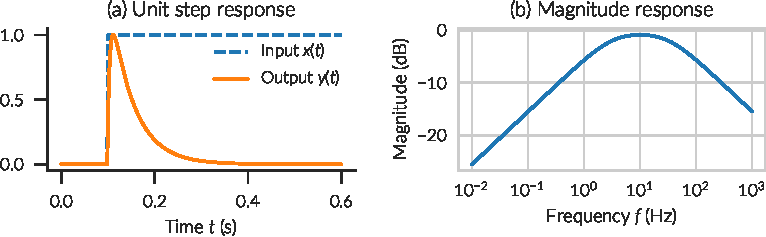
\includegraphics{figures/differentiator}
    \caption{Differentiator with $\tau_1 = \SI{5}{\milli\second}$ and $\tau_2 = \SI{50}{\milli\second}$. (a) Response of the differentiator to a unit step input. The output has been normalized to the maximum. (b) Magnitude response for sinusoidal inputs with different frequencies.}\label{fig:differentiator}
\end{figure}
\begin{figure}
    \centering
    \begin{tikzpicture}[nef]
        \graph {
            x/"$\vc x$" [ens] -> ["$+1, \syntau=\tau_1$", bend left] y/"$\vc y$" [ens];
            x -> ["$-1, \syntau=\tau_2$" below, bend right] y;
        };
    \end{tikzpicture}
    \caption{Implementation of a differentiator with the NEF\@. The connection labels state the transform and synaptic time constants with $\tau_1 < \tau_2$.}\label{fig:differentiator-net}
\end{figure}


\section{Integrator}
Integrators are important components in many NEF models because they allow to store values over some timespan in neural activity.
An integrator is described by the differential equation
\begin{equation}
    \od{\vc x(t)}{t} = \vc u(t)
\end{equation}
where $\vc u(t)$ is the external input to the integrator.
Applying principle 3 of the NEF tells us that the input has to be scaled by the synaptic time constant $\tausyn$.
Furthermore, a recurrent connection feeding the output of the integrator back to itself is needed.
To get a stable representations over a sufficient time window, it is best to use a long time constant like $\tausyn = \SI{0.1}{\second}$ which is the range measured for the TODO neurotransmitter.
Due to neural noise and distortion error, the represented value can drift over time.
Adding more neurons to the integrator will make it more stable.
\begin{figure}
    \centering
    \begin{tikzpicture}[nef]
        \graph {
            u/"$\vc u$" -> ["$\syntau$" above] x/"$\vc x$" [ens];
            x -> [out=300, in=60, distance=40pt] x;
        };
    \end{tikzpicture}
    \caption{Implementation of an integrator with the NEF.}\label{fig:integrator-net}
\end{figure}
TODO figures


\section{Gated memory buffer}
While the integrator enables us to store a value over time, it does not allow for particularly quick updating.
A quicker update can be achieved by adding a difference ensemble (TODO figure).
By scaling the difference with a factor the updating speed can be regulated.
However, too large values will lead to oscillations in the integrator.
Note that in this case feeding a null vector to the difference ensemble will clear out the memory instead of keeping the current value.
Thus, the input the integrator needs to be gated.
This can be done by inhibiting the neurons of the difference ensemble to keep the current value in the integrator.

\section{Thresholding ensembles}\label{sec:thresholding}
Often one needs to apply a threshold to value, i.e.\ implement the function
\begin{equation}
    f(x) = \left\{ \begin{array}{ll}
            0 & x < 0 \\
            x & x \geq 0
        \end{array} \right.
    \text{,}
\end{equation}
or compute the Heaviside step function
\begin{equation}
    \Heavi(x) = \left\{ \begin{array}{ll}
            0 & x < 0 \\
            1 & x \geq 0
        \end{array} \right.
    \text{.}
\end{equation}
Both of these functions are non-differentiable at 0.
The Heaviside function is even discontinuous at that spot.
These properties make it problematic to implement this function with a standard NEF ensemble.
Nevertheless, a good approximations of these functions can be achieved by aligning the neuron's tuning curves according to the shape of these functions.

Instead of choosing encoders randomly as $-1$ and $1$, all encoders are set to $1$ and all intercepts are chosen from $x \in [0; 1]$.
Choosing the intercept distribution of this interval appropriately can further increase the accuracy.
An exponential distribution that clusters intercepts close to 0 performs best.
Note that this is even better than setting all intercepts to 0 as this gives more variation in the tuning curves.
The uniform distribution often does not produce intercepts close enough to the threshold value which leads to an increased effective threshold.

TODO figures

\section{Product}
A product of two scalar numbers $x$ and $y$ could be computed by feeding them into separate dimensions of a two-dimensional ensemble and decoding out the product.
A \SI{37}{\percent} more accurate implementation (with the same number of neurons) is, however, possible (TODO ref) by rewriting the product with squares as
\begin{equation}
    xy = \frac{1}{4}\del{x^2 + 2xy + y^2} - \frac{1}{4}\del{x^2 - 2xy + y^2} = \frac{1}{4}\del{x + y}^2 - \frac{1}{4}\del{x - y}^2 \text{.}
\end{equation}
The neural implementation of this equation is straight-forward (TODO figure).

Multiple scalar product networks can be combined to compute element-wise vector products.
By summing across those element-wise products a dot product can be computed.
Product networks are also used in the computation of circular convolution as binding operation in the Semantic Pointer Architecture (TODO ref section).
